\subsubsection{UC8 - Ricerca funzione}
\begin{figure}[h]
	\centering
	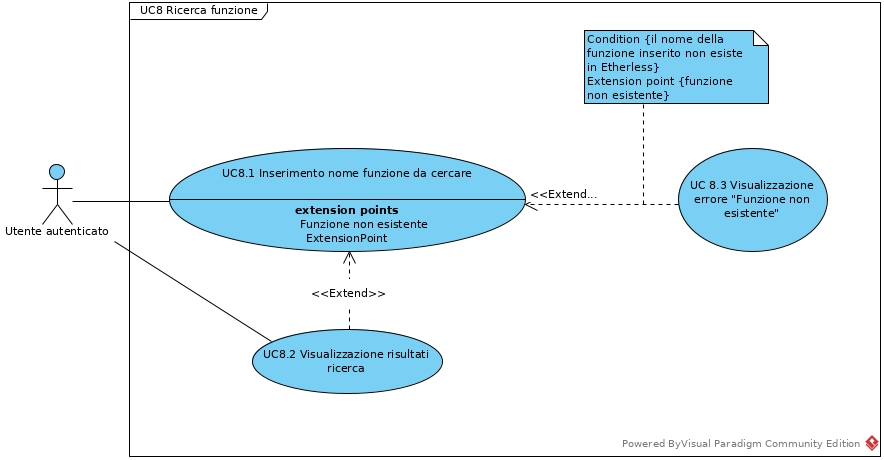
\includegraphics[width=\linewidth]{res/img/UC8.jpg}
	\caption{Diagramma UC8 - Ricerca funzione}
\end{figure}
\begin{itemize}
	\item \textbf{Attori primari:} Utente autenticato;
	\item \textbf{Descrizione:} l'utente autenticato ricerca per nome i dettagli di una specifica funzione caricata da un utente sviluppatore sulla rete \textit{Etherless};
	\item \textbf{Pre-condizioni:} l'utente ha effettuato l'accesso ad \textit{Etherless} e vuole ricercare una funzione specifica mediante l'apposito comando;
	\item \textbf{Post-condizioni:} il sistema visualizzerà a schermo i dettagli della funzione ricercata o un messaggio di errore se la funzione non è stata trovata;
	\item \textbf{Scenario principale:}
	\begin{enumerate}
		\item L'utente scriverà un comando da \textit{CLI\glos} composto nel seguente modo:
		\begin{itemize}
			\item nome del comando "find";
			\item nome della funzione da ricercare.
		\end{itemize}
        \item L'utente visualizzerà la funzione ricercata e i suoi dettagli.
	\end{enumerate}
\end{itemize}
